\section{Results}\label{sec:results}

\subsection{Detection}
On HAI, the four detectors detect 89--92\,\% of the 50 attacks at 0.34--0.42 false alarms per hour, with median delays of 6--15\,s (\cref{tab:detection}). On PCL-Sim, event recall is 76--96\,\%; point-wise recall is low because the PI controllers partly compensate the manipulations. In ten HAI attacks the score crosses $\theta$ 1--4\,s before the labelled onset, which suggests that documented onsets lag slightly; we keep the documented labels. Localization is evaluated on detected attacks (\nhaitesthrOnealarmZero{} (attack, detector) units on HAI, \nsimtesthrOnealarmZero{} on PCL-Sim); deadline metrics count missed detections as failures.

\begin{table}[t]
\centering\scriptsize
\caption{Detection performance (mean$\pm$sd over 3 seeds; no point adjustment). Event recall: alarm within the attack or 60\,s after it. FA/h: false-alarm runs per hour of attack-free data.}\label{tab:detection}
\resizebox{\linewidth}{!}{%
\begin{tabular}{@{}llcccccc@{}}
\toprule
Data & Detector & P & R & F1 & Event rec. & Delay [s] & FA/h\\
\midrule
PCL-Sim & Linear & 0.79 & 0.17 & 0.28 & 0.96 & 6 & 1.38\\
 & MLP & 0.81$\pm$0.06 & 0.07$\pm$0.04 & 0.13$\pm$0.07 & 0.76$\pm$0.03 & 226$\pm$176 & 0.31$\pm$0.03\\
 & CNN & 0.83$\pm$0.03 & 0.19$\pm$0.02 & 0.31$\pm$0.02 & 0.89$\pm$0.00 & 46$\pm$38 & 0.96$\pm$0.06\\
 & GRU & 0.77$\pm$0.02 & 0.42$\pm$0.01 & 0.54$\pm$0.01 & 0.93$\pm$0.00 & 7$\pm$1 & 0.89$\pm$0.05\\
\midrule
HAI 21.03 & Linear & 0.79$\pm$0.00 & 0.60$\pm$0.00 & 0.68$\pm$0.00 & 0.92 & 6 & 0.42$\pm$0.03\\
 & MLP & 0.75$\pm$0.01 & 0.50$\pm$0.02 & 0.60$\pm$0.02 & 0.90 & 15$\pm$1 & 0.36$\pm$0.04\\
 & CNN & 0.74$\pm$0.01 & 0.48$\pm$0.01 & 0.58$\pm$0.01 & 0.89$\pm$0.01 & 14$\pm$0 & 0.34$\pm$0.01\\
 & GRU & 0.78$\pm$0.00 & 0.55$\pm$0.00 & 0.65$\pm$0.00 & 0.90 & 14$\pm$1 & 0.36$\pm$0.02\\
\bottomrule
\end{tabular}}
\end{table}


\subsection{Localization at the alarm (RQ1)}
\Cref{tab:loc_hai,tab:loc_sim} report loop localization for all configurations.
\begin{itemize}
\item \emph{PI-CAX is the most accurate explainer.} It ranks the attacked loop first in \lochaiPICAXalarmZerosinglehrOne{} of detected attacks on HAI and \locsimPICAXalarmZerosinglehrOne{} on PCL-Sim, significantly better than every other configuration (Holm $p\pctesthaialarmmaxp$ on HAI and $p\pctestsimalarmmaxp$ on PCL-Sim, $n=\pctesthaialarmn$ and \pctestsimalarmn).
\item \emph{Among score attributions,} \LX{} is the most accurate on HAI (\lochaiLXalarmZerosinglehrOne; IG \lochaiIGalarmZerosinglehrOne, Holm $p=\phaitesthrOnealarmZeroIGtea$), whereas on PCL-Sim most score attributions lie within two points of each other (\LX{} \locsimLXalarmZerosinglehrOne, \LX-bg \locsimLXbgalarmZerosinglehrOne). H1 is therefore only partially supported.
\item \emph{Chance and structure.} A random ranking would rank a target loop first in \chancehaihrOne{} of the same units on both benchmarks (HAI \chancehaihrOne, PCL-Sim \chancesimhrOne). Exact Shapley values over correlation clusters (CLX) or random groups of the loop sizes (RPX) reach only 0.45/0.25 on HAI and 0.27/0.54 on PCL-Sim (all Holm $p<10^{-10}$ against \LX), so the gain of loop attribution comes from control structure, not grouping per se (H4 supported).
\item \emph{Best-guess timing} \citep{fung2024attributions} does not help: on HAI it is worse than practical timing for every method except saliency, which is unchanged (\LX{} \lochaiLXbestguesssinglehrOne), because many manipulations take tens of seconds to affect the process.
\end{itemize}

\begin{table}[t]
\centering\scriptsize
\caption{Loop localization on HAI 21.03 (pooled over 4 detectors; mean over attacks, seeds averaged). Bold: best in column. Single-shot unless marked \TEA.}\label{tab:loc_hai}
\resizebox{\linewidth}{!}{%
\begin{tabular}{@{}lcccccccc@{}}
\toprule
& \multicolumn{6}{c}{HR@1} & HR@3 & nRank\\\cmidrule(lr){2-7}\cmidrule(lr){8-8}\cmidrule(lr){9-9} Method & best-guess & alarm & +60\,s & +60\,s\,\TEA & +180\,s & +180\,s\,\TEA & +60\,s\,\TEA & +60\,s\,\TEA\\
\midrule
RE & 0.49 & 0.71 & 0.48 & 0.61 & \textbf{0.35} & 0.57 & 0.89 & 0.09\\
SM & 0.43 & 0.43 & 0.32 & 0.44 & 0.22 & 0.44 & 0.67 & 0.27\\
IG & 0.50 & 0.75 & 0.56 & \textbf{0.72} & 0.33 & 0.70 & 0.93 & \textbf{0.06}\\
KernelSHAP-eq & 0.47 & 0.70 & 0.50 & 0.64 & 0.22 & 0.60 & 0.90 & 0.09\\
KernelSHAP-1024 & 0.48 & 0.74 & 0.51 & 0.69 & 0.28 & 0.65 & 0.92 & 0.07\\
LIME-eq & 0.49 & 0.75 & 0.55 & 0.70 & 0.26 & 0.66 & 0.93 & 0.07\\
LIME-1024 & 0.49 & 0.76 & 0.56 & 0.69 & 0.31 & 0.66 & 0.93 & 0.07\\
Fung ens. & \textbf{0.60} & 0.76 & 0.56 & \textbf{0.72} & 0.34 & \textbf{0.71} & 0.92 & 0.07\\
CLX (clusters) & 0.31 & 0.45 & 0.39 & 0.38 & 0.20 & 0.38 & 0.79 & 0.18\\
RPX (random) & 0.17 & 0.25 & 0.19 & 0.21 & 0.16 & 0.17 & 0.68 & 0.26\\
\LX-bg & 0.55 & 0.74 & 0.58 & 0.71 & 0.31 & 0.65 & \textbf{0.94} & \textbf{0.06}\\
\textbf{\LX{} (ours)} & 0.47 & \textbf{0.79} & \textbf{0.60} & 0.70 & 0.30 & 0.64 & \textbf{0.94} & \textbf{0.06}\\
\bottomrule
\end{tabular}}
\end{table}

\begin{table}[t]
\centering\scriptsize
\caption{Loop localization on PCL-Sim (pooled over 4 detectors; mean over attacks, seeds averaged). Bold: best in column. Single-shot unless marked \TEA.}\label{tab:loc_sim}
\resizebox{\linewidth}{!}{%
\begin{tabular}{@{}lcccccccc@{}}
\toprule
& \multicolumn{6}{c}{HR@1} & HR@3 & nRank\\\cmidrule(lr){2-7}\cmidrule(lr){8-8}\cmidrule(lr){9-9} Method & best-guess & alarm & +60\,s & +60\,s\,\TEA & +180\,s & +180\,s\,\TEA & +60\,s\,\TEA & +60\,s\,\TEA\\
\midrule
RE & 0.43 & 0.86 & 0.44 & 0.80 & 0.41 & 0.80 & 0.96 & 0.07\\
SM & 0.44 & 0.65 & 0.43 & 0.70 & 0.40 & 0.69 & 0.95 & 0.10\\
IG & \textbf{0.68} & 0.86 & 0.66 & 0.84 & 0.55 & 0.83 & 0.96 & 0.06\\
KernelSHAP-eq & 0.46 & 0.80 & 0.47 & 0.71 & 0.40 & 0.69 & 0.90 & 0.13\\
KernelSHAP-1024 & 0.50 & 0.84 & 0.50 & 0.80 & 0.43 & 0.77 & 0.93 & 0.09\\
LIME-eq & 0.42 & 0.82 & 0.46 & 0.72 & 0.40 & 0.70 & 0.91 & 0.12\\
LIME-1024 & 0.50 & 0.85 & 0.52 & 0.82 & 0.45 & 0.81 & 0.95 & 0.07\\
Fung ens. & 0.48 & 0.87 & 0.49 & 0.82 & 0.45 & 0.82 & 0.97 & 0.06\\
PI-CAX & -- & \textbf{0.89} & \textbf{0.79} & \textbf{0.87} & \textbf{0.72} & \textbf{0.87} & \textbf{0.99} & \textbf{0.04}\\
CLX (clusters) & 0.12 & 0.27 & 0.16 & 0.23 & 0.14 & 0.23 & 0.78 & 0.31\\
RPX (random) & 0.35 & 0.54 & 0.35 & 0.58 & 0.32 & 0.58 & 0.90 & 0.16\\
\LX-bg & 0.54 & 0.87 & 0.60 & 0.85 & 0.50 & 0.83 & 0.96 & 0.06\\
\LX & 0.57 & 0.85 & 0.53 & 0.82 & 0.46 & 0.80 & 0.95 & 0.07\\
\bottomrule
\end{tabular}}
\end{table}


\subsection{After the alarm: propagation and temporal accumulation (RQ2)}
Single-shot score attributions degrade quickly after the alarm, for every method (\cref{fig:overtime}). On HAI, \LX{} falls from \lochaiLXalarmZerosinglehrOne{} at the alarm to \lochaiLXalarmSixZerosinglehrOne{} after 60\,s and \lochaiLXalarmOneEightZerosinglehrOne{} after 180\,s; on PCL-Sim from \locsimLXalarmZerosinglehrOne{} to \locsimLXalarmSixZerosinglehrOne{} and \locsimLXalarmOneEightZerosinglehrOne. Once controllers react, the largest residuals move to loops that compensate for the manipulated one, which adds a mechanism to the timing effect of \citet{fung2024attributions}.
\begin{itemize}
\item \emph{\TEA{} recovers part of the loss for every method} (H2 supported). \LX+\TEA{} reaches \lochaiLXalarmSixZeroteahrOne{} (HAI) and \locsimLXalarmSixZeroteahrOne{} (PCL-Sim) at 60\,s (Holm $p=\phaitesthrOnealarmSixZeroLXsingle$ and $p=\psimtesthrOnealarmSixZeroLXsingle$ against single-shot), and single-shot top-1 outputs that change between consecutive explanations in 12--48\,\% of cases become 95--100\,\% consistent (\cref{tab:quality}). With \TEA, the leading score attributions are within a few points of each other: on HAI \LX{} is not significantly different from IG, \LX-bg, the Fung ensemble, LIME-1024 or KernelSHAP-1024; on PCL-Sim IG and \LX-bg are slightly but significantly better (Supplementary Table~S2).
\item \emph{PI-CAX degrades far less.} Single-shot, it still reaches \lochaiPICAXalarmSixZerosinglehrOne{} (HAI) and \locsimPICAXalarmSixZerosinglehrOne{} (PCL-Sim) at 60\,s; with \TEA, \lochaiPICAXalarmSixZeroteahrOne{} and \locsimPICAXalarmSixZeroteahrOne, significantly better than every other configuration (Holm $p\pctesthaisixtymaxp$ and $p\pctestsimsixtymaxp$). With \TEA, the attacked loop is among PI-CAX's top three in \lochaiPICAXalarmSixZeroteahrThree{} and \locsimPICAXalarmSixZeroteahrThree{} of cases.
\end{itemize}

\begin{figure}[t]
\centering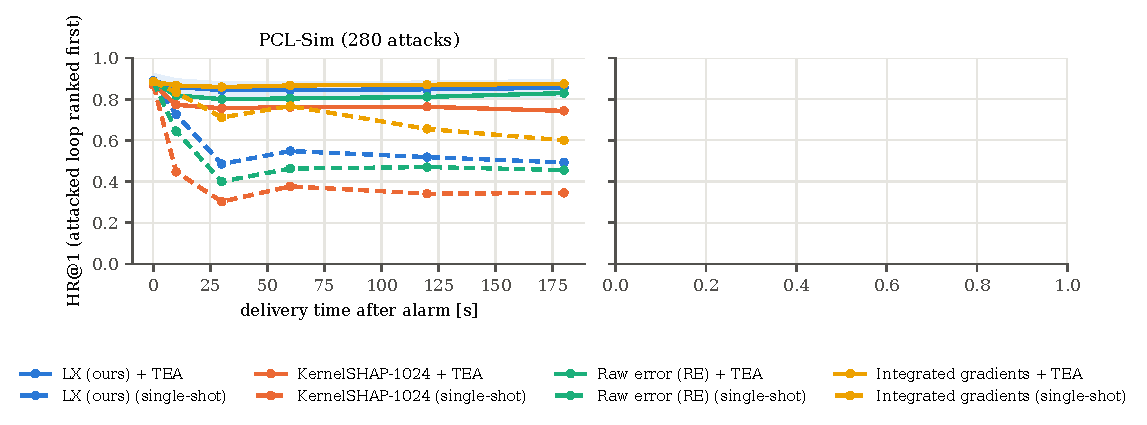
\includegraphics[width=\linewidth]{figures/hr1_over_time.pdf}
\caption{Top-1 loop localization versus delivery time after the alarm (solid: with \TEA; dashed: single-shot; band: 95\,\% bootstrap CI for \LX+\TEA). Score attributions decay as the attack propagates through coupled loops; PI-CAX decays least.}\label{fig:overtime}
\end{figure}


\subsection{Why the physical prior works}
\Cref{tab:pcab} switches PI-CAX's components off one at a time (seed 0, all four detectors). Removing the persistence--oscillation decoupling reduces it to the level of the score attributions (HAI: \pcabhaiNoCausalalarm{} at the alarm and \pcabhaiNoCausalsingle{} single-shot at 60\,s). Removing the precision weighting and loop gating, the operating envelope or the counterfactual check changes accuracy by at most 0.04. The advantage therefore comes from one physical hypothesis: the manipulated loop departs \emph{persistently} from its normal cross-loop relations, while compensating loops \emph{oscillate}. Score attributions cannot express this distinction, because they only ask how much each loop contributes to the current score.

\begin{table}[t]
\centering\scriptsize
\caption{PI-CAX component ablation: loop HR@1 (single-shot at the alarm / single-shot at +60\,s / +60\,s with \TEA; seed 0, four detectors pooled).}\label{tab:pcab}
\begin{tabular}{@{}lcc@{}}
\toprule
Configuration & HAI 21.03 & PCL-Sim\\
\midrule
Full PI-CAX & \pcabhaiFullalarm{} / \pcabhaiFullsingle{} / \pcabhaiFulltea & \pcabsimFullalarm{} / \pcabsimFullsingle{} / \pcabsimFulltea\\
-- persistence/oscillation decoupling & \pcabhaiNoCausalalarm{} / \pcabhaiNoCausalsingle{} / \pcabhaiNoCausaltea & \pcabsimNoCausalalarm{} / \pcabsimNoCausalsingle{} / \pcabsimNoCausaltea\\
-- precision weighting and loop gating & \pcabhaiNoManifoldalarm{} / \pcabhaiNoManifoldsingle{} / \pcabhaiNoManifoldtea & \pcabsimNoManifoldalarm{} / \pcabsimNoManifoldsingle{} / \pcabsimNoManifoldtea\\
-- operating envelope & \pcabhaiNoEnvelopealarm{} / \pcabhaiNoEnvelopesingle{} / \pcabhaiNoEnvelopetea & \pcabsimNoEnvelopealarm{} / \pcabsimNoEnvelopesingle{} / \pcabsimNoEnvelopetea\\
-- counterfactual check & \pcabhaiNoTieralarm{} / \pcabhaiNoTiersingle{} / \pcabhaiNoTiertea & \pcabsimNoTieralarm{} / \pcabsimNoTiersingle{} / \pcabsimNoTiertea\\
none (smoothed residuals only) & \pcabhaiNonealarm{} / \pcabhaiNonesingle{} / \pcabhaiNonetea & \pcabsimNonealarm{} / \pcabsimNonesingle{} / \pcabsimNonetea\\
\bottomrule
\end{tabular}
\end{table}

\paragraph{Hard-to-explain attacks} \Cref{tab:strata} stratifies HAI by the type of manipulated variable, read from the target-controller code of the official attack table (strata of 3--\stratcombn{} attacks; descriptive only). Controller-output (CV) attacks move a recorded actuator and are localized well by most methods (0.79 at the alarm for IG, KernelSHAP-1024, \LX-bg and \LX). Setpoint (SP) attacks are the hardest for score attributions: the setpoint is largely invisible in the data, and every score attribution falls to \stratSPteamin--\stratSPteamax{} at 60\,s even with \TEA. PI-CAX localizes them in \stratSPPICAXtea{} of cases, plausibly because a hidden setpoint change produces exactly the persistent PV/CV departure it looks for. Its weakest stratum is SP attacks combined with a PV spoof (\stratSPPVPICAXtea{} at 60\,s, $n=\stratSPPVn$), possibly because the spoofed PV hides the persistent departure.

\begin{table}[htbp]
\centering\scriptsize
\caption{HAI 21.03 loop HR@1 by manipulated variable type, read from the target-controller code of the official attack table (attacks detected by at least one detector; single-shot at the alarm / +60\,s with \TEA; pooled over 4 detectors). Strata are small; descriptive only.}\label{tab:strata}
\resizebox{\linewidth}{!}{%
\begin{tabular}{@{}lccccccc@{}}
\toprule
Manipulated variable & attacks & RE & IG & KernelSHAP-1024 & \LX-bg & \LX & PI-CAX\\
\midrule
SP only & 8 & 0.69 / 0.38 & 0.66 / 0.52 & 0.66 / 0.46 & 0.65 / 0.47 & 0.73 / 0.46 & 0.93 / 0.98\\
SP + PV spoof & 4 & 0.50 / 0.31 & 0.56 / 0.65 & 0.58 / 0.60 & 0.65 / 0.62 & 0.71 / 0.62 & 0.75 / 0.52\\
CV only & 8 & 0.69 / 0.74 & 0.79 / 0.79 & 0.79 / 0.78 & 0.79 / 0.84 & 0.79 / 0.79 & 0.99 / 0.98\\
CV + PV spoof & 3 & 0.94 / 0.89 & 0.97 / 0.92 & 0.92 / 0.78 & 0.97 / 0.94 & 1.00 / 0.89 & 1.00 / 1.00\\
combined (2 scenarios) & 23 & 0.73 / 0.66 & 0.77 / 0.76 & 0.75 / 0.74 & 0.74 / 0.73 & 0.80 / 0.74 & 0.93 / 0.96\\
\bottomrule
\end{tabular}}
\end{table}


\subsection{Deadlines, latency and cost (RQ3)}
\Cref{tab:deadline_hai,tab:deadline_sim} and \cref{fig:dcl} account for detection delay, explainer latency and the correctness of the delivered explanation.
\begin{itemize}
\item \emph{HAI.} DCL@1 at $D=60$\,s is \dclhaiPICAXdclfixedSixZerotea{} for PI-CAX+\TEA{} against \dclhaiLXdclfixedSixZerotea{} for \LX+\TEA{} and at most \dclhaiIGdclfixedSixZerotea{} for any other configuration (Holm $p\pctesthaidclmaxp$, $n=\pctesthaidcln$). It is bounded by event recall, so PI-CAX delivers a correct loop for most detected attacks within a minute of onset. No score attribution differs significantly from \LX{} in DCL@1 at 60\,s (H3 not supported for DCL).
\item \emph{PCL-Sim.} The correct loop is ranked first before the hazard deadline minus a 30\,s action reserve in \dclsimLXdclhazhztea{} (\LX+\TEA), \dclsimPICAXdclhazhztea{} (PI-CAX+\TEA) and \dclsimIGdclhazhztea{} (IG+\TEA) of hazardous cases. No explainer improves this rate materially, because the failures are dominated by detection: of the \intimeFail{} failing (attack, detector, seed) cases of \LX+\TEA, \intimeFailUndelivered{} (\intimeFailUndeliveredPct\,\%) were detected too late for any explanation to be delivered. Conditional on delivery, the top-ranked loop is correct in \intimeDeliveredLX{} (\LX), \intimeDeliveredPICAX{} (PI-CAX) and \intimeDeliveredIG{} (IG) of cases.
\item \emph{Latency.} \LX{} costs $2^L$ evaluations per explanation (512 on HAI, 64 on PCL-Sim), i.e.\ \latsimLXlinear--\latsimLXcnn\,ms on PCL-Sim and \lathaiLXlinear--\lathaiLXcnn\,ms on HAI on one thread (\cref{tab:latency}); PI-CAX needs 16 evaluations (median 1.4--1.7\,ms during the runs, \cref{tab:deadline_hai,tab:deadline_sim}). Both are deterministic and need no gradients; IG is cheaper than \LX{} but requires gradient access.
\item \emph{Slower hardware.} We did not measure on embedded devices. Multiplying every measured latency by an assumed factor of 10 or 100 changes DCL@1 at $D=30$\,s by at most 0.04 for all configurations except \LX-bg on HAI (4096 evaluations), which drops from \slowhaixoneLXbgthirty{} to \slowhaixhundredLXbgthirty. At these model sizes, latency is not the binding constraint; detection delay is.
\item \emph{ShaTS-sensor} needs $\approx\!2\cdot20\,d^2$ evaluations ($\evalshaiShaTS$ on HAI), \lathaiShaTScnn\,s for the CNN. At the alarm on HAI it localizes \shatshaicnnHR{} of attacks against \shatshaicnnLXHR{} for \LX{} on the same incidents (CNN, seed 0, $n=\shatshaicnnN$; linear: \shatshailinearHR{} vs.\ \shatshailinearLXHR), at roughly 250--280 times the cost.
\end{itemize}

\begin{figure}[t]
\centering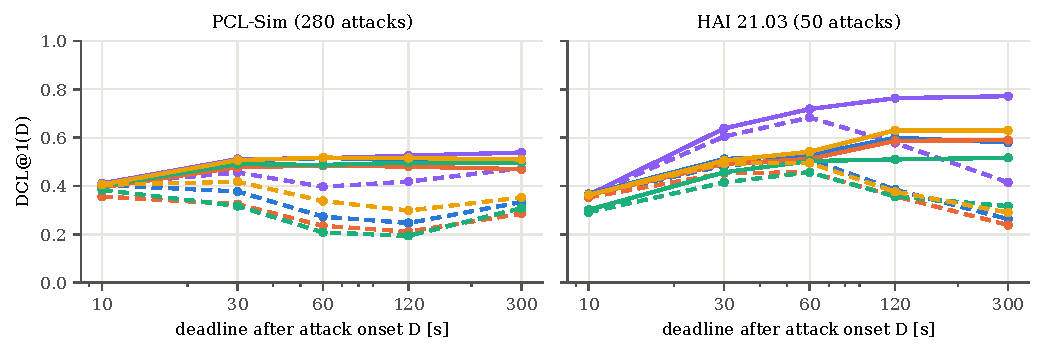
\includegraphics[width=\linewidth]{figures/dcl.pdf}
\caption{Deadline-conditioned localization DCL@1($D$) (colours as in \cref{fig:overtime}; solid: \TEA; dashed: single-shot). Missed detections and undelivered explanations count as failures, so curves are bounded by event recall.}\label{fig:dcl}
\end{figure}

\begin{table}[t]
\centering\scriptsize
\caption{Deadline-conditioned localization on HAI 21.03 (T = with \TEA). Latency: median measured per explanation during the runs (1 thread, pooled over detectors); Evals: detector evaluations per explanation.}\label{tab:deadline_hai}
\resizebox{\linewidth}{!}{%
\begin{tabular}{@{}lccccccc@{}}
\toprule
Method & \multicolumn{4}{c}{DCL@1($D$)} & DCL@3 & Lat.\,[ms] & Evals\\ & 30\,s\,T & 60\,s & 60\,s\,T & 120\,s\,T & 60\,s\,T & & \\
\midrule
RE & 0.46 & 0.46 & 0.50 & 0.51 & 0.68 & 0.5 & 1\\
SM & 0.32 & 0.31 & 0.32 & 0.39 & 0.49 & 1.0 & 1\\
IG & 0.51 & 0.49 & 0.54 & 0.63 & 0.68 & 3.4 & 32\\
KernelSHAP-eq & 0.47 & 0.41 & 0.48 & 0.55 & 0.67 & 20.4 & 512\\
KernelSHAP-1024 & 0.49 & 0.46 & 0.51 & 0.59 & 0.68 & 40.9 & 1024\\
LIME-eq & 0.50 & 0.48 & 0.52 & 0.60 & 0.68 & 38.1 & 512\\
LIME-1024 & 0.51 & 0.50 & 0.52 & 0.60 & 0.69 & 85.9 & 1024\\
Fung ens. & 0.54 & 0.51 & 0.54 & 0.62 & 0.72 & 43.8 & 514\\
PI-CAX & \textbf{0.64} & \textbf{0.68} & \textbf{0.72} & \textbf{0.76} & \textbf{0.78} & 1.7 & 16\\
CLX (clusters) & 0.30 & 0.34 & 0.32 & 0.34 & 0.61 & 14.2 & 512\\
RPX (random) & 0.16 & 0.17 & 0.19 & 0.17 & 0.52 & 13.0 & 512\\
\LX-bg & 0.51 & 0.51 & 0.53 & 0.60 & 0.70 & 200.2 & 4096\\
\LX & 0.51 & 0.51 & 0.53 & 0.60 & 0.70 & 28.2 & 512\\
\bottomrule
\end{tabular}}
\end{table}

\begin{table}[t]
\centering\scriptsize
\caption{Deadline-conditioned localization on PCL-Sim (T = with \TEA). Latency: median measured per explanation during the runs (1 thread, pooled over detectors); Evals: detector evaluations per explanation. In-time: hazard deadline minus a 30\,s operator reserve, hazardous attacks only.}\label{tab:deadline_sim}
\resizebox{\linewidth}{!}{%
\begin{tabular}{@{}lcccccccccc@{}}
\toprule
Method & \multicolumn{4}{c}{DCL@1($D$)} & DCL@3 & \multicolumn{2}{c}{In-time@1} & In-time@3 & Lat.\,[ms] & Evals\\ & 30\,s\,T & 60\,s & 60\,s\,T & 120\,s\,T & 60\,s\,T & single & T & T & & \\
\midrule
RE & 0.49 & 0.21 & 0.49 & 0.50 & \textbf{0.53} & 0.17 & 0.41 & \textbf{0.54} & 0.3 & 1\\
SM & 0.47 & 0.21 & 0.46 & 0.47 & \textbf{0.53} & 0.19 & 0.40 & \textbf{0.54} & 0.8 & 1\\
IG & \textbf{0.51} & \textbf{0.34} & \textbf{0.52} & \textbf{0.52} & \textbf{0.53} & \textbf{0.33} & \textbf{0.50} & \textbf{0.54} & 2.2 & 32\\
KernelSHAP-eq & 0.40 & 0.23 & 0.40 & 0.40 & 0.48 & 0.25 & 0.40 & 0.51 & 2.4 & 64\\
KernelSHAP-1024 & 0.48 & 0.24 & 0.48 & 0.48 & 0.52 & 0.22 & 0.43 & 0.51 & 24.2 & 1024\\
LIME-eq & 0.42 & 0.21 & 0.42 & 0.42 & 0.50 & 0.20 & 0.38 & 0.48 & 1.8 & 64\\
LIME-1024 & 0.50 & 0.24 & 0.50 & 0.50 & \textbf{0.53} & 0.22 & 0.46 & 0.52 & 15.4 & 1024\\
Fung ens. & 0.50 & 0.23 & 0.50 & 0.50 & \textbf{0.53} & 0.21 & 0.44 & \textbf{0.54} & 3.2 & 66\\
CLX (clusters) & 0.10 & 0.09 & 0.10 & 0.10 & 0.41 & 0.10 & 0.14 & 0.38 & 1.6 & 64\\
RPX (random) & 0.32 & 0.17 & 0.33 & 0.35 & 0.51 & 0.17 & 0.29 & 0.50 & 1.5 & 64\\
\LX-bg & \textbf{0.51} & 0.28 & \textbf{0.52} & \textbf{0.52} & \textbf{0.53} & 0.29 & 0.49 & \textbf{0.54} & 7.3 & 512\\
\textbf{\LX{} (ours)} & \textbf{0.51} & 0.27 & \textbf{0.52} & 0.51 & \textbf{0.53} & 0.28 & 0.48 & 0.53 & 1.6 & 64\\
\bottomrule
\end{tabular}}
\end{table}

\begin{table}[t]
\centering\tiny
\caption{Explanation latency on one CPU thread of an otherwise idle machine (median over 10 incidents $\times$ 5 repetitions, ms; ShaTS: 2 incidents, 1 repetition). Evals: detector evaluations per explanation.}\label{tab:latency}
\resizebox{\linewidth}{!}{%
\begin{tabular}{@{}llrrrrr@{}}
\toprule
Data & Method & Evals & Linear & MLP & CNN & GRU\\
\midrule
\bottomrule
\end{tabular}}
\end{table}


\subsection{Explanation quality beyond accuracy}
\Cref{tab:quality} reports further properties.
\begin{itemize}
\item \emph{Faithfulness.} Deletion AUCs at the alarm are similar for all accurate methods (0.16--0.22), including PI-CAX; saliency and the structure controls are worse.
\item \emph{Stability under input noise.} On HAI, PI-CAX's single explanations are the most sensitive to Gaussian input perturbation (top-3 Jaccard \qhaiPICAXnoise{} on HAI, against \qhaiLXnoise{} for \LX{} and 0.70 for KernelSHAP-1024), because its persistence statistics use only ten samples. Exact attributions are also less stable than fixed-seed sampling estimators. \TEA{} mitigates both in operation.
\item \emph{Tags.} Within the top loop, H-\LX{} ranks a manipulated tag first in \qhaiLXtagone{} (HAI) and \qsimLXtagone{} (PCL-Sim) of attacks; PI-CAX's tag ranking reaches \qhaiPICAXtagone{} and \qsimPICAXtagone{}, the best of all methods.
\end{itemize}

\begin{table}[t]
\centering\scriptsize
\caption{Explanation quality. Temporal agreement: share of consecutive explanations (5\,s apart, first 120\,s) with the same top-1 loop. Noise Jaccard: top-3 overlap under Gaussian input noise ($\sigma=0.1$) at alarm and +60\,s. Deletion: area under the normalised score curve when loops are restored to the training mean in ranked order (lower is better), at the alarm. Tag HR@$k$: rank of a manipulated tag among all tags at the alarm (for \LX: H-\LX{} refinement); HAI excludes P2 setpoint targets that are invisible in the data.}\label{tab:quality}
\resizebox{\linewidth}{!}{%
\begin{tabular}{@{}llcccccc@{}}
\toprule
Data & Method & \multicolumn{2}{c}{Temporal top-1 agr.} & Noise Jacc.@3 & Deletion$\downarrow$ & Tag HR@1 & Tag HR@3\\ & & single & \TEA & & & & \\
\midrule
PCL-Sim & RE & 0.53 & 0.99 & 0.49 & 0.18 & 0.38 & \textbf{0.76}\\
 & SM & 0.52 & 0.99 & 0.53 & 0.28 & 0.20 & 0.53\\
 & IG & 0.71 & \textbf{1.00} & 0.53 & 0.18 & 0.44 & 0.74\\
 & KernelSHAP-eq & \textbf{0.77} & 0.99 & 0.71 & 0.19 & 0.43 & 0.69\\
 & KernelSHAP-1024 & 0.74 & 0.99 & 0.62 & 0.18 & 0.44 & 0.73\\
 & LIME-eq & 0.74 & 0.99 & 0.71 & 0.21 & 0.41 & 0.69\\
 & LIME-1024 & 0.70 & 0.99 & 0.59 & 0.20 & 0.44 & 0.73\\
 & Fung ens. & 0.59 & 0.99 & 0.60 & \textbf{0.17} & 0.28 & 0.75\\
 & CLX (clusters) & 0.61 & 0.99 & 0.64 & 0.34 & 0.05 & 0.27\\
 & RPX (random) & 0.63 & 0.98 & \textbf{0.76} & 0.26 & 0.00 & 0.08\\
 & \LX-bg & 0.66 & 0.99 & 0.55 & 0.22 & -- & --\\
 & \textbf{\LX{} (ours)} (H-\LX) & 0.64 & 0.99 & 0.51 & 0.21 & \textbf{0.45} & \textbf{0.76}\\
\midrule
HAI 21.03 & RE & 0.58 & 0.95 & 0.59 & 0.18 & 0.23 & 0.40\\
 & SM & 0.62 & 0.95 & 0.44 & 0.45 & 0.10 & 0.34\\
 & IG & 0.67 & \textbf{0.97} & 0.59 & 0.17 & 0.28 & 0.41\\
 & KernelSHAP-eq & \textbf{0.69} & \textbf{0.97} & 0.73 & 0.19 & 0.29 & 0.39\\
 & KernelSHAP-1024 & 0.68 & \textbf{0.97} & 0.70 & 0.18 & 0.31 & 0.41\\
 & LIME-eq & 0.67 & \textbf{0.97} & 0.65 & 0.17 & 0.30 & 0.41\\
 & LIME-1024 & 0.68 & \textbf{0.97} & 0.62 & 0.17 & 0.31 & 0.41\\
 & Fung ens. & 0.66 & 0.96 & 0.54 & \textbf{0.16} & \textbf{0.36} & 0.48\\
 & CLX (clusters) & \textbf{0.69} & 0.96 & 0.75 & 0.26 & 0.00 & 0.00\\
 & RPX (random) & 0.63 & 0.95 & \textbf{0.76} & 0.33 & 0.00 & 0.00\\
 & \LX-bg & 0.68 & 0.96 & 0.57 & \textbf{0.16} & -- & --\\
 & \textbf{\LX{} (ours)} (H-\LX) & 0.68 & 0.96 & 0.56 & 0.17 & 0.31 & \textbf{0.49}\\
\bottomrule
\end{tabular}}
\end{table}


\subsection{Robustness (RQ4)}\label{sec:ablation}
\Cref{tab:phase2} summarises the robustness experiments (CNN detector, seed 0, unless noted).
\begin{itemize}
\item \emph{Reference gap.} \LX{} is insensitive to $\Delta_{\mathrm{ref}}\in\{32,60,120,300\}$\,s on PCL-Sim. On HAI the default of 60\,s is best at the alarm (\ptwohairefBLXsingleZerohrOne, against \ptwohairefDLXsingleZerohrOne--\ptwohairefCLXsingleZerohrOne{} for the other gaps), a difference of a few attacks; we did not tune the gap on test data. PI-CAX does not use the reference.
\item \emph{Sensor noise.} With the alarm threshold kept from clean data, Gaussian noise saturates the detector (precision \ptwohainoiseAcleandetprecision{} on HAI), so we recalibrate $\sigma$ and $\theta$ on equally noisy validation data with frozen weights, as an operator would. Localization then degrades for the score attributions on HAI (\LX+\TEA{} \ptwohainoiseALXteaSixZerohrOne{} and \ptwohainoiseBLXteaSixZerohrOne{} at $\sigma_n=0.1/0.3$, against \ptwohairefBLXteaSixZerohrOne{} without noise), and no score attribution differs significantly from \LX{} (H5a not supported). PI-CAX, with its normalising statistics recalibrated on the same data, stays at \ptwohainoiseAPICAXteaSixZerohrOne{} and \ptwohainoiseBPICAXteaSixZerohrOne. \emph{Without} that recalibration it collapses (\pcfrozenhaiAtea{} and \pcfrozenhaiBtea), so its statistics must be refitted whenever sensor noise changes. On PCL-Sim, noise mainly delays detection, and all methods reach 0.91--0.95 at 60\,s with \TEA.
\item \emph{Decoy.} A small bias on the PV of an innocent loop captures the top rank in at most \ptwosimdecoyLXteaSixZerodecoytopOne{} of attacks for any method with \TEA{} (PI-CAX \ptwosimdecoyPICAXteaSixZerodecoytopOne). A non-adaptive decoy of this size is ineffective against all methods, so it cannot discriminate between them (H5b not supported).
\end{itemize}

\begin{table}[t]
\centering\tiny
\caption{Ablations and robustness (HR@1 unless noted; ``alarm'': single shot at the alarm; ``+60\,T'': 60\,s after the alarm with \TEA). Reference-gap and noise rows: CNN detector, seed 0. Noise rows: Gaussian noise of standard deviation $\sigma_n$ (standardised units) added to the test and validation data, with $\sigma$ and $\theta$ recalibrated on the noisy validation data (model weights frozen; PI-CAX's normalising statistics are recalibrated on the same data). Decoy rows: linear and CNN detectors, 3 seeds; decoy@1 is the share of attacks in which the innocent decoy loop is ranked first.}\label{tab:phase2}
\resizebox{\linewidth}{!}{%
\begin{tabular}{@{}llcccccccccc@{}}
\toprule
Data & Condition & \multicolumn{2}{c}{PI-CAX} & \multicolumn{2}{c}{\LX} & \multicolumn{2}{c}{IG} & \multicolumn{2}{c}{KS-1024} & \multicolumn{2}{c}{RE}\\ & & alarm & +60\,T & alarm & +60\,T & alarm & +60\,T & alarm & +60\,T & alarm & +60\,T\\
\midrule
HAI & $\Delta_{\mathrm{ref}}$=32\,s & 0.96 & 0.96 & 0.67 & 0.67 & 0.64 & 0.67 & 0.64 & 0.71 & 0.73 & 0.69\\
HAI & $\Delta_{\mathrm{ref}}$=60\,s (default) & 0.96 & 0.96 & 0.73 & 0.67 & 0.64 & 0.67 & 0.69 & 0.69 & 0.73 & 0.69\\
HAI & $\Delta_{\mathrm{ref}}$=120\,s & 0.96 & 0.96 & 0.71 & 0.64 & 0.69 & 0.67 & 0.69 & 0.67 & 0.73 & 0.69\\
HAI & $\Delta_{\mathrm{ref}}$=300\,s & 0.96 & 0.96 & 0.64 & 0.62 & 0.64 & 0.71 & 0.64 & 0.71 & 0.73 & 0.69\\
HAI & $\sigma_n$=0.1, recal. & 0.82 & 0.86 & 0.64 & 0.61 & 0.61 & 0.70 & 0.66 & 0.68 & 0.64 & 0.73\\
HAI & $\sigma_n$=0.3, recal. & 0.67 & 0.84 & 0.51 & 0.56 & 0.56 & 0.60 & 0.56 & 0.63 & 0.56 & 0.44\\
\midrule
PCL-Sim & $\Delta_{\mathrm{ref}}$=32\,s & 0.86 & 0.84 & 0.79 & 0.76 & 0.78 & 0.75 & 0.78 & 0.78 & 0.82 & 0.79\\
PCL-Sim & $\Delta_{\mathrm{ref}}$=60\,s (default) & 0.86 & 0.84 & 0.80 & 0.76 & 0.80 & 0.77 & 0.79 & 0.78 & 0.82 & 0.79\\
PCL-Sim & $\Delta_{\mathrm{ref}}$=120\,s & 0.86 & 0.84 & 0.80 & 0.76 & 0.82 & 0.78 & 0.82 & 0.79 & 0.82 & 0.79\\
PCL-Sim & $\Delta_{\mathrm{ref}}$=300\,s & 0.86 & 0.84 & 0.81 & 0.78 & 0.82 & 0.78 & 0.82 & 0.78 & 0.82 & 0.79\\
PCL-Sim & $\sigma_n$=0.1, recal. & 0.92 & 0.91 & 0.93 & 0.91 & 0.93 & 0.92 & 0.93 & 0.93 & 0.94 & 0.91\\
PCL-Sim & $\sigma_n$=0.3, recal. & 0.94 & 0.94 & 0.94 & 0.93 & 0.95 & 0.95 & 0.95 & 0.94 & 0.95 & 0.93\\
\midrule
PCL-Sim & no decoy: HR@1 & 0.87 & 0.86 & 0.84 & 0.80 & 0.84 & 0.82 & 0.83 & 0.77 & 0.85 & 0.78\\
PCL-Sim & decoy: HR@1 & 0.89 & 0.87 & 0.86 & 0.81 & 0.85 & 0.83 & 0.84 & 0.78 & 0.85 & 0.79\\
PCL-Sim & decoy: decoy@1 & 0.03 & 0.03 & 0.03 & 0.05 & 0.03 & 0.04 & 0.03 & 0.05 & 0.04 & 0.05\\
\bottomrule
\end{tabular}}
\end{table}


\subsection{Leakage from random window splits (RQ5)}
A gradient-boosting classifier on window features (last value, mean and standard deviation of every tag) of the HAI attack files reaches F1 $=\leakRandomFOne\pm\leakRandomFOnesd$ with a random 70/30 split, but F1 $=\leakBlockedFOne\pm\leakBlockedFOnesd$ with a chronological, attack-disjoint split (train on test1--3, evaluate on test4--5; 5 seeds). Overlapping windows of the same attack instance on both sides of a random split inflate F1 by $\approx$0.37 (H6 supported); explanations of models evaluated this way inherit the optimism.

\begin{table}[t]
\centering\scriptsize
\caption{Outcome of the pre-specified hypotheses and of the post hoc PI-CAX comparison.}\label{tab:hyp}
\begin{tabular}{@{}lp{5.2cm}p{5.6cm}@{}}
\toprule
H & Statement & Outcome\\
\midrule
H1 & \LX{} localizes better than tag-level methods & partially: best score attribution at the alarm on HAI; not better than IG, nor than \LX-bg on PCL-Sim\\
H2 & \TEA{} improves accuracy after the alarm and temporal stability & supported (both benchmarks, all methods)\\
H3 & \LX+\TEA{} has deterministic cost and the best DCL / in-time rate & cost: supported; DCL: not supported\\
H4 & control structure beats data-driven / random grouping & supported ($p<10^{-10}$)\\
H5a & \LX+\TEA{} degrades less under sensor noise & not supported\\
H5b & a decoy captures top-1 less often with \LX+\TEA & not supported (decoy ineffective against all methods)\\
H6 & random splits inflate detection & supported (F1 \leakRandomFOne{} vs.\ \leakBlockedFOne)\\
\midrule
post hoc & PI-CAX vs.\ all other configurations & better at the alarm and at +60\,s on both benchmarks and in DCL@1(60\,s) on HAI; tied in the PCL-Sim in-time rate; needs recalibration under changed noise\\
\bottomrule
\end{tabular}
\end{table}
